\documentclass[10pt,a4paper]{article}
\usepackage[utf8]{inputenc}
\usepackage{amsmath}
\usepackage{amsfonts}
\usepackage{amssymb}
\usepackage{german}
\usepackage{fancyhdr}
\usepackage{graphicx}
\usepackage{geometry}
\usepackage{color}
\usepackage[usenames,dvipsnames]{xcolor}
\usepackage{DejaVuSans}
\usepackage[T1]{fontenc}
\usepackage{listings}
\definecolor{dkgreen}{rgb}{0,0.6,0}
\definecolor{gray}{rgb}{0.5,0.5,0.5}
\definecolor{mauve}{rgb}{0.58,0,0.82}
\definecolor{backcolour}{rgb}{0.95,0.95,0.92}
\definecolor{stackreferencegreen}{rgb}{0,0.69,0.313}
\definecolor{heapreferencered}{rgb}{0.753,0,0}

\lstset{
  language={[Sharp]C},
  backgroundcolor=\color{backcolour},
  framexleftmargin=3mm,
  framexrightmargin=3mm,
  framextopmargin=3mm,
  framexbottommargin=3mm,
  alsolanguage=CIL,
  aboveskip=3mm,
  belowskip=3mm,
  showstringspaces=false,
  columns=flexible,
  basicstyle={\small\ttfamily},
  numbers=none,
  numberstyle=\tiny\color{gray},
  keywordstyle=\color{blue},
  commentstyle=\color{dkgreen},
  stringstyle=\color{mauve},
  breaklines=true,
  breakatwhitespace=true,
  tabsize=3
}
\renewcommand*{\familydefault}{\sfdefault}
\geometry{verbose,a4paper,tmargin=35mm,bmargin=35mm,lmargin=25mm,rmargin=25mm}
\author{Dominik Heeb \& Fabian Keller}
\title{Findings}
\pagestyle{fancy}
\fancyhead{}
\fancyhead[L]{Findings - Dynamic Parallel Checker}
\fancyhead[R]{Domink Heeb \& Fabian Keller}
\fancyfoot{}
\fancyfoot[R]{Seite \thepage}
\begin{document}
\begin{titlepage}
	\begin{Huge}
		\begin{center}
				Findings \\Dynamic Parallel Checker\\[2.0cm]
		\end{center}
	\end{Huge}
	
	\begin{center}
		\begin{Large}
				by Dominik Heeb \& Fabian Keller\\[1.0cm]
		\end{Large}
	\end{center}
\end{titlepage}

\newpage
\tableofcontents 
\newpage

\section{Einleitung}
\begin{flushleft}
Dieses Dokument beinhaltet Findings(Erkenntnisse) welche während der Arbeit am 'Dynamic Parallel Checker' aufgefunden wurden.
\end{flushleft}
\section{Findings zu Mono.Cecil}
\subsection{Lokale Variablen}
\subsubsection{Ausgangslage}
\begin{flushleft}
Um den Stack zur Laufzeit verwerten zu können, aber trotzdem die Gültigkeit nach der Verarbeitung sicherzustellen, muss der Stack zum Teil abgebaut und wieder aufgebaut werden. Um die Werte die oben auf dem Stack liegen, nicht zu verlieren, werden lokale Variablen verwendet.
Das Problem bei der Arbeit mit lokalen Variablen ist, dass diese von der Instrumentation, sowie auch vom Hauptprogram verwendet werden können. Wichtig ist es daher sicherzustellen, dass die Variablen nicht die selben sind, wie die vom Hauptprogram verwendeten.
Mono.Cecil erlaubt es einem während der Instrumentation neue Variablen einzufügen, dabei muss aber das Verhalten von Cecil beachtet werden.
\end{flushleft}
\subsubsection{Erkenntnis}
\begin{flushleft}
Um die Grösse der Instrumentation klein zu halten, wurde entschieden nicht für jeden Instrumentationsvorgang neue Variablen zu definieren, sondern diese wiederzuverwerten. Dadurch soll der Overhead der Instrumentation reduziert werden.
Bei der Arbeit mit Cecil wurde dann eine globale Definition eingesetzt, welche im Code verwendet wurde.
Dabei zeigte sich jedoch dass die Klasse VariableDefinition per Seiteneffekt bearbeitet wird. Durch das hinzufügen in einer Methode wird der Klasse ein Name fest eingetragen. Durch weitere Methoden wird dieser fortlaufen überschrieben und erst beim Speichern des Assembly geschrieben. Dadurch kann es zu grossen Fehlern kommen, da die Variablennamen nicht mehr stimmen.
Daher muss die Definition der Variable pro Methode neu erstellt werden (siehe Bild unten)
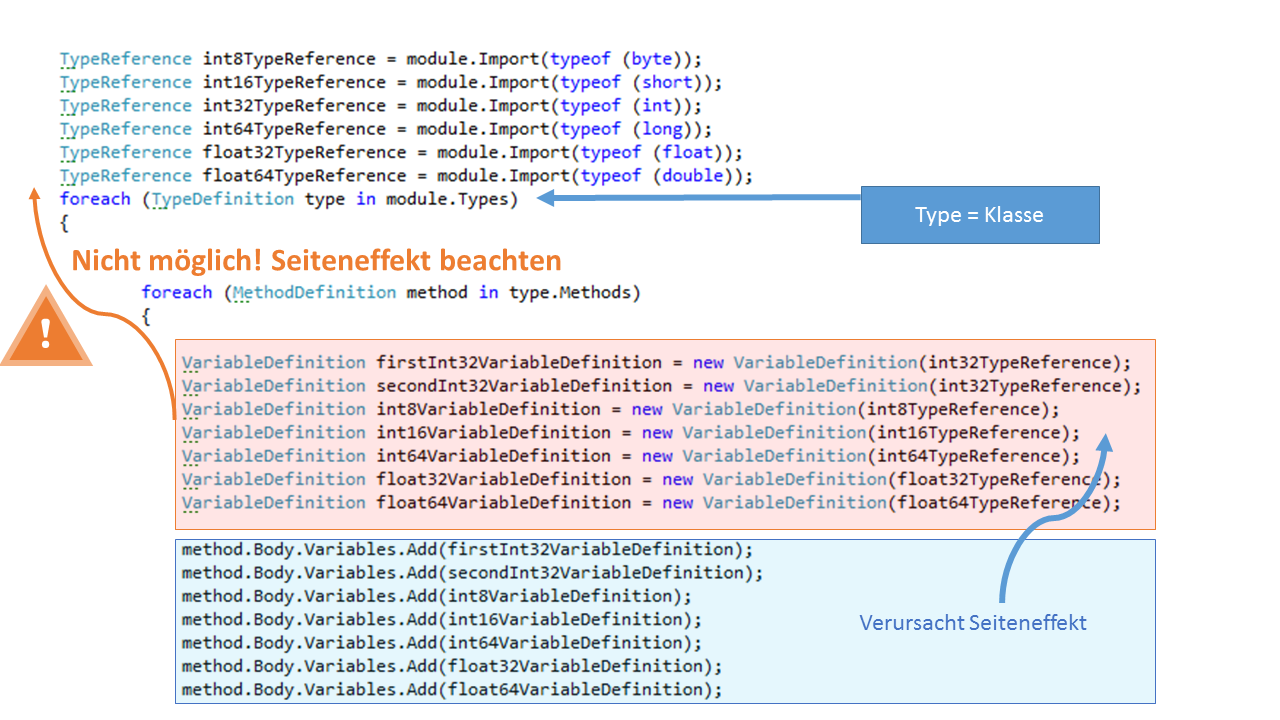
\includegraphics[width=14cm, clip]{pictures/VariableDefinition.png}
\end{flushleft} \newpage
\subsection{Short Branches}
\subsubsection{Ausgangslage}
\begin{flushleft}
Bei der Instrumentation von Code ist es wichtig zu beachten das für einige Befehle wie (try/catch/finally usw.) Sprungmarken(Branches) verwendet. Diese Verweisen auf eine bestimmte Zeile innerhalb des IL Codes.
\begin{lstlisting} 
br IL_0003 /*Branch zu Zeile IL_0003*/
call *****
IL_0003: ret
\end{lstlisting}
Durch die Instrumentation werden diese Zeilen zum Teil auseinandergeschoben und daher die Werte nicht mehr korrekt. Mono.Cecil hilft einem dabei und passt die Werte neu an.
Jedoch muss die Grösse des Codes beachtet werden.
\end{flushleft}
\subsubsection{Erkenntnis}
\begin{flushleft}
Wenn der IL Code nicht gross ist, werden für die Branch Nummern short Werte verwendet.
Daher muss dies während der Instrumentation beachtet werden. Denn short wird relativ schnell überschritten, dies wird standardmässig von Cecil nicht weiter beachtet. Daher kommt es in so einem Fall zu grösseren Problemen, da die Referenzen nicht mehr stimmen.
Mono.Cecil stellt dafür zwei Methoden zur Verfügung. Diese müssen vor und nach der Instrumentation verwendet werden, um dieses Problem zu beheben.
\begin{lstlisting} 
method.Body.SimplifyMacros(); // convert every br.s (short branch) to a normal branch
/*.....Code Instrumentation.....*/
method.Body.OptimizeMacros(); // Convert the normal branches back to short branches if possible
\end{lstlisting}
Dieser Befehl muss pro Methode welche instrumentiert wird aufgerufen werden.
\end{flushleft}
\newpage
\section{Findings zur CLR}
\subsection{Refernce-Type/Value-Type}
\subsubsection{Ausgangslage}
\begin{flushleft}
In Programmiersprachen werden Datentypen in zwei Kategorien eingeteilt: Reference- oder Value- Types. Als Value-Types werden die Basistypen wie (int, float, char, short, usw.) gehandelt. Zusätzlich zu den Basisdatentypen werden auch Structs (in .Net) als Value-Type gehandelt. String jedoch ist ein Reference-Type.\\
Der Unterschied dieser Kategorien bezieht sich auf das Handling im Memory. Value-Types werden als effektive Werte auf dem Stack gespeichert.\\
Reference-Types werden als Referenz auf dem Stack gespeichert. Die Werte befinden sich auf dem Heap.\\
Dieser Unterschied muss während der Instrumentation beachtet werden. Denn bei Reference-Types gibt es zwei Referenzen: 
\begin{enumerate}
\item Die {\color{stackreferencegreen} Referenz} auf das Feld, welches den Reference-Type beinhaltet.
\item Die {\color{heapreferencered}Referenz} auf den Reference-Type im Heap.
\end{enumerate}
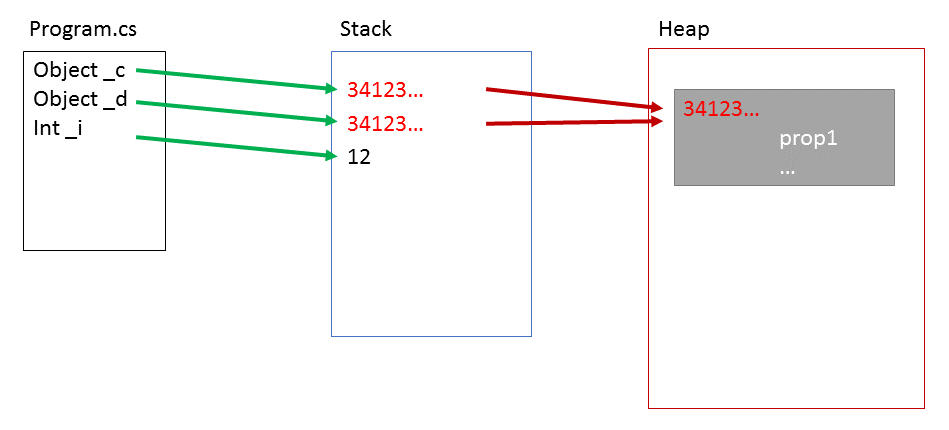
\includegraphics[width=14cm, clip]{pictures/ValueReferenceType.png}
\end{flushleft}
\subsubsection{Erkenntnis}
\begin{flushleft}
Bei der Realisation des Dynamic Parallel Checkers ist dieser Fakt essentiell. Bei der Detektion einer Race Condition, kann diese bei der Referenz auf den Stack, sowie auf das referenzierte Objekt im Heap entstehen.
Daher müssen für das monitoren der Zugriffe immer beide Referenzen beachtet werden.
Im IL Code können die zwei Referenzen über zwei Befehle ausgelesen werden.
\begin{lstlisting} 
  /* Beispiel mit Static Fields. Verhaltet sich mit anderen Field-Typen gleich */
IL_0059:  ldsflda    class TestProgram.NewObject TestProgram.Program::_obj
  /* Referenz auf das Feld im Stack liegt Top-Of-Stack */
IL_005e:  ldsfld     class TestProgram.NewObject TestProgram.Program::_obj
  /* Referenz auf das Feld im Heap liegt Top-Of-Stack oder Wert eines Value-Types */
\end{lstlisting}
\end{flushleft}
\newpage
\section{Findings Dynamic Parallel Checker}
\subsection{Asynchrone vs. synchrone Architektur}
\subsubsection{Ausgangslage}
\begin{flushleft}
Der Dynamic Parallel Checker kann mit einer Asynchronen, sowie einer synchronen Architektur konzeptionell realisiert werden. Beide Architekturen haben Vor- / sowie Nachteile. Daher müssen sie gegeneinander aufgewogen werden.\\
Eine Asynchrone Architektur instrumentiert den IL Code so dass die Werte über einen Kommunikationskanal (z.B. Named Pipe) übertragen wird und vom Hauptprogram verarbeitet.
Die synchrone Architektur instrumentiert den Code so, dass neben dem lesen der Werte auch der Check übernommen wird. Dabei ist das Programm blockierend.
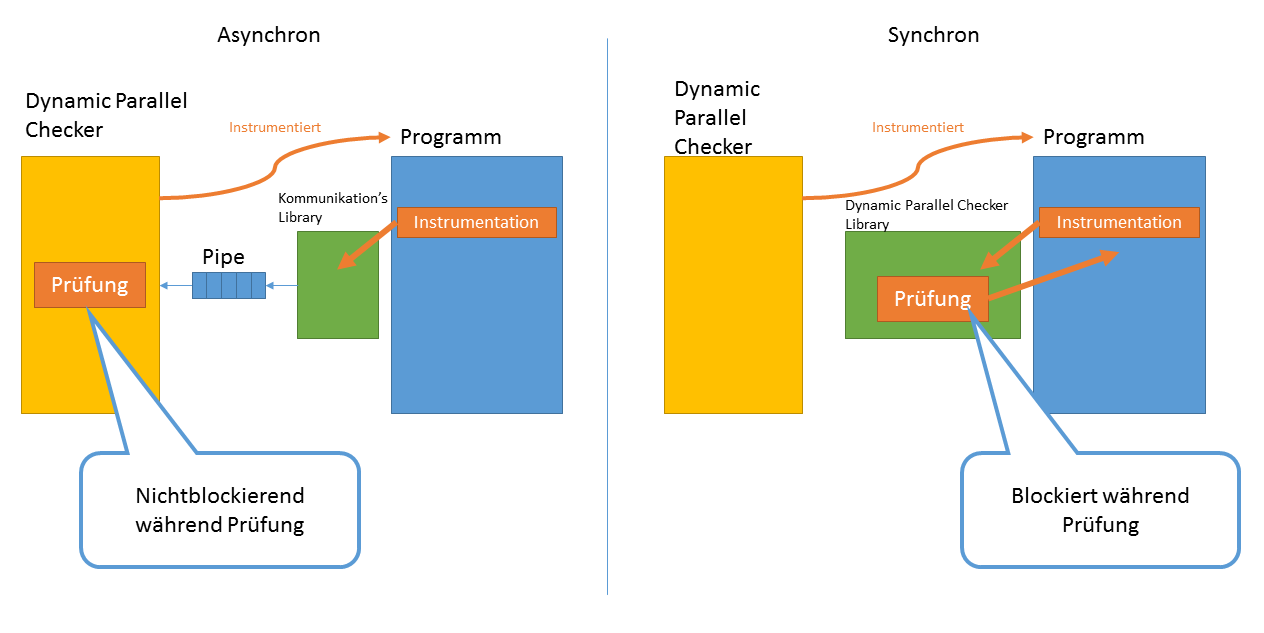
\includegraphics[width=16cm, clip]{pictures/AsnycSyncArchitecture.png}
\end{flushleft}
\subsubsection{Erkenntnis}
\begin{flushleft}
Bei aktuellen Programmierkonzepten werden blockierende Archtiekturen vermieden, um die Nutzungsperformance hochzuhalten. Jedoch muss im Beispiel des Dynamic Parallel Checker beachtet werden, um was für Datenmengen es sich handelt. Die Prüfung in der asynchronen Architektur kann ohne Blockierungsmechanismus nicht mit dem Programm mithalten. Dadurch wird bei grossen Softwareprojekten die Pipe immer weiter gefüllt, bis der Speicher nicht mehr ausreicht. Ein anderes Argument gegen die asynchrone Architektur ist der zeitliche Aspekt. Die Prüfung wird über einen längeren Zeitpunkt immer weiter Entfernt vom Zeitpunkt des Fehlers sein. So könnte es theoretisch vorkommen, dass eine Race Condition auftritt, der DPC es aber erst 5-10min später meldet, da er mit der Überprüfung so weit hinter her ist.\\
{\huge \color{red} TODO:Vergleich async vs. Sync}
\end{flushleft}
\end{document}
